\documentclass[11pt]{article}
\usepackage[margin=1in]{geometry}
\usepackage{graphicx}
\usepackage{enumitem}
\usepackage{parskip}

\title{Admin Onboarding}
\author{}
\date{}

\begin{document}

\maketitle

\section*{Current Status}
Verified on March 16, 2026 against the live Supabase-backed portal.

Smoke-tested admin workflows:
\begin{itemize}
  \item login and dashboard load
  \item settings access
  \item billing access
  \item admin saved-view create and delete
  \item engineer-only tools remained absent from the admin experience
\end{itemize}

\section*{What Admin Is For}
Admin runs the school-day operations layer.

Admin owns:
\begin{itemize}
  \item cohorts and schedules
  \item task assignment
  \item family follow-up
  \item billing follow-up workflow
  \item saved views
  \item announcements
  \item operational oversight across staff, TA, and instructor work
\end{itemize}

Admin does not own:
\begin{itemize}
  \item engineer break-glass
  \item feature flags
  \item change freeze
  \item integration maintenance mode
  \item engineer incident controls
\end{itemize}

\section*{Core Boundaries}
Admin can:
\begin{itemize}
  \item access every normal portal section
  \item manage \texttt{staff}, \texttt{ta}, and \texttt{instructor} accounts
  \item work with billing and exports
  \item manage operational tasks and announcements
  \item use approvals, escalations, saved views, archive and restore actions, and capacity forecasting
  \item work contact history and internal billing follow-up
\end{itemize}

Admin cannot:
\begin{itemize}
  \item manage \texttt{admin} or \texttt{engineer} accounts
  \item use engineer support tooling
  \item view or operate the schema inspector
  \item run system remediation actions
\end{itemize}

\section*{Screens}
\subsection*{Admin Dashboard}
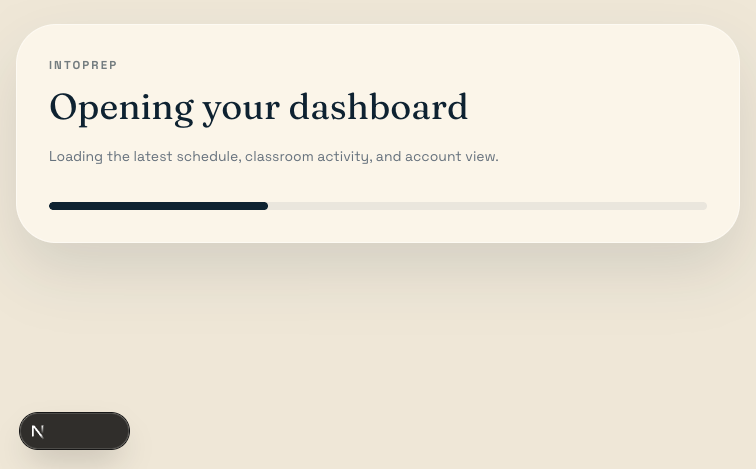
\includegraphics[width=\textwidth]{assets/admin-dashboard.png}

\subsection*{Admin Billing}
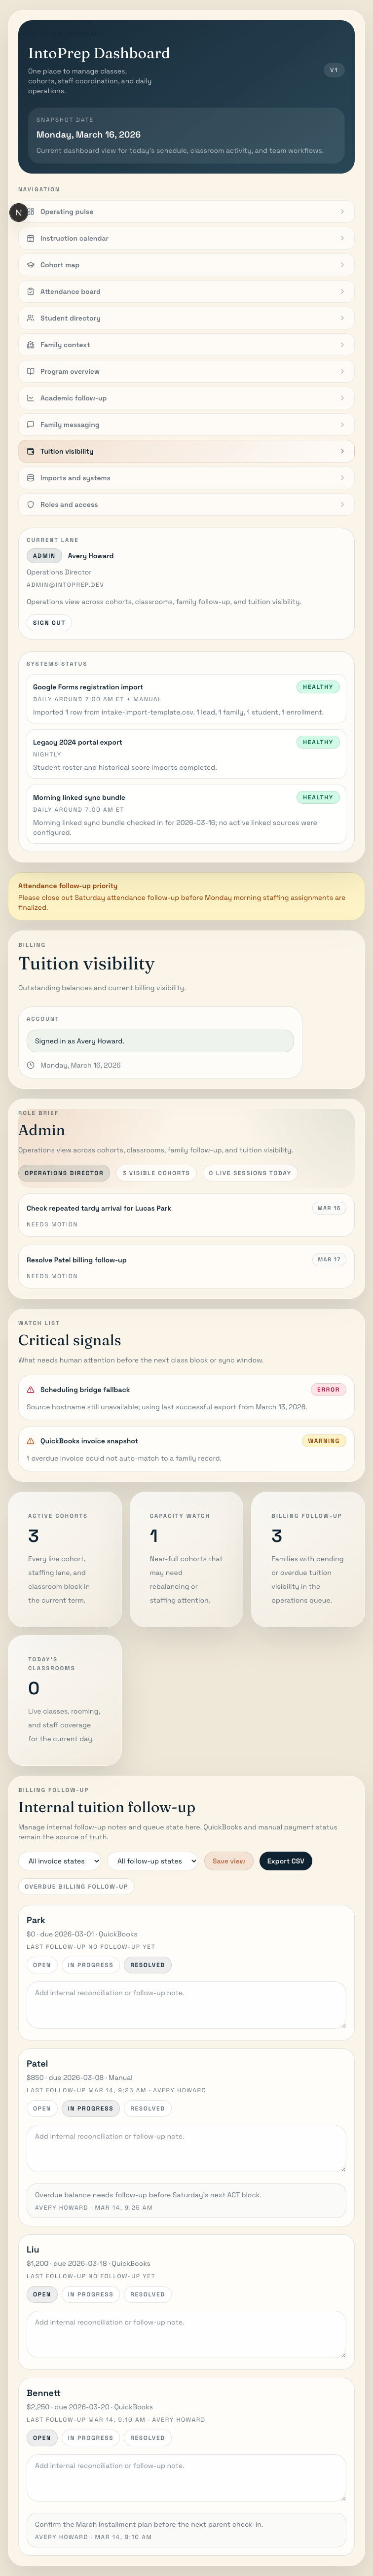
\includegraphics[width=\textwidth]{assets/admin-billing.png}

\subsection*{Admin Settings}

\includegraphics[width=\textwidth]{assets/admin-settings.png}

\section*{First Login Walkthrough}
\begin{enumerate}
  \item Sign in at \texttt{/login}.
  \item Start on ``Operating pulse''.
  \item Review:
  \begin{itemize}
    \item follow-up queue
    \item pending staff escalations
    \item staff and TA announcements
    \item onboarding watch
    \item capacity forecasting
  \end{itemize}
  \item Open ``Tuition visibility'' and confirm the billing queue is visible.
  \item Open ``Roles and access'' and confirm only staff, TA, and instructor management surfaces are available.
\end{enumerate}

\section*{Daily Workflow}
\subsection*{1. Start With Operations Pulse}
Review:
\begin{itemize}
  \item cohort capacity
  \item outstanding classroom issues
  \item billing follow-up workload
  \item pending escalations and approvals
  \item onboarding gaps for staff, TA, and instructor
\end{itemize}

\subsection*{2. Work The Follow-Up Queue}
Use the tasking panel to:
\begin{itemize}
  \item create operational tasks
  \item assign ownership
  \item set due dates
  \item track status
\end{itemize}

Typical admin task types:
\begin{itemize}
  \item billing follow-up
  \item family communication
  \item attendance follow-up
  \item missing scores
  \item cohort staffing
\end{itemize}

\subsection*{3. Review Billing Daily}
Open ``Tuition visibility''.

Use billing to:
\begin{itemize}
  \item review overdue or pending invoices
  \item update internal follow-up state
  \item add notes for follow-up context
  \item keep finance work coordinated without changing source-of-truth invoice state
\end{itemize}

\subsection*{4. Manage People Safely}
Open ``Roles and access''.

Use this area to:
\begin{itemize}
  \item provision staff, TA, and instructor accounts
  \item suspend or reactivate those accounts
  \item manage cohort assignments for TA and instructor
  \item review operational audit trails
\end{itemize}

\subsection*{5. Coordinate The Team}
Use admin announcements for operational notices.

Good examples:
\begin{itemize}
  \item attendance follow-up priority
  \item rooming changes
  \item score-entry deadlines
  \item upcoming billing handoffs
\end{itemize}

\section*{Complete Capability Map}
Admin is the business-operations owner inside the portal.

Use admin for:
\begin{itemize}
  \item operational dashboard review
  \item user management for staff, TA, and instructor
  \item cohort and program operations
  \item bulk cohort actions
  \item archive and restore for cohorts and programs
  \item approvals and escalations
  \item billing exports and billing follow-up
  \item saved views
  \item parent contact history
  \item staff-facing internal announcements
  \item onboarding watch and capacity forecasting
\end{itemize}

Do not use admin for:
\begin{itemize}
  \item engineer break-glass
  \item feature flags
  \item change freeze
  \item schema inspection
  \item integration remediation and platform-repair tooling
\end{itemize}

\section*{How To Save And Reopen A Queue}
\begin{enumerate}
  \item Open the section you care about, such as billing or academics.
  \item Apply the filters you use repeatedly.
  \item Save the filtered view.
  \item Reopen it later from the saved-views list on the dashboard.
\end{enumerate}

Verified in smoke testing:
\begin{itemize}
  \item admin saved-view create worked
  \item admin saved-view delete worked
\end{itemize}

\section*{How To Use Billing Follow-Up}
\begin{enumerate}
  \item Open ``Tuition visibility''.
  \item Find the invoice or family needing action.
  \item Review current status, due date, and last follow-up state.
  \item Add the new follow-up note.
  \item Update the follow-up state:
  \begin{itemize}
    \item \texttt{open}
    \item \texttt{in\_progress}
    \item \texttt{resolved}
  \end{itemize}
  \item If issue needs someone else, assign a task from the admin dashboard.
\end{enumerate}

\section*{How To Work Escalations And Approvals}
\begin{enumerate}
  \item Review escalations and approval requests from the dashboard or the related ops panels.
  \item Open the request or escalation and read the handoff context before acting.
  \item Decide whether the item should be:
  \begin{itemize}
    \item acknowledged
    \item approved
    \item rejected
    \item closed after action
  \end{itemize}
  \item Complete the operational action in the correct workflow surface.
  \item Leave the system in a clean status so staff and TA know what happened.
\end{enumerate}

\section*{How To Manage Cohorts And Programs}
\begin{enumerate}
  \item Open ``Cohort map'' or ``Program overview''.
  \item Review capacity, enrollment, rooming, and staffing context.
  \item Use conflict warnings before finalizing schedule or cohort changes.
  \item Use archive or restore for lifecycle changes instead of deleting records outright.
  \item Use bulk operations only when you are confident the cohort impact is correct.
\end{enumerate}

\section*{How To Use Contact History}
\begin{enumerate}
  \item Open the family or billing workflow surface.
  \item Review the existing outreach timeline first.
  \item Add the new contact event with the source and outcome.
  \item Keep notes short and operational so the next person can continue the thread cleanly.
\end{enumerate}

\section*{How To Use Announcements}
\begin{enumerate}
  \item Draft the message as an internal operations notice.
  \item Target only the roles that need it.
  \item Set the active window if timing matters.
  \item Remove or expire the message when it is no longer operationally relevant.
\end{enumerate}

\section*{How To Read Capacity Forecasting}
\begin{itemize}
  \item near-full cohorts:
  rebalance early before room or staffing pressure becomes a problem.
  \item underfilled cohorts:
  review whether intake, placement, or schedule changes are needed.
  \item onboarding watch:
  use it with the forecast to spot where new staff, TA, or instructor coverage may be missing.
\end{itemize}

\section*{How To Review Role Access}
\begin{enumerate}
  \item Open ``Roles and access''.
  \item Search for the user.
  \item Confirm the role and status are correct.
  \item Update only staff, TA, or instructor accounts from here.
  \item Use password reset or assignment actions when onboarding a user.
\end{enumerate}

\section*{Guardrails}
\begin{itemize}
  \item admin cannot manage admin or engineer accounts
  \item admin cannot use engineer-only support or incident tools
  \item exports and billing changes are audited
  \item destructive operational lifecycle changes should prefer archive or close flows instead of hard deletion
\end{itemize}

\section*{Verified Behavior}
Verified in the live browser pass:
\begin{itemize}
  \item admin login succeeded
  \item admin dashboard loaded correctly
  \item ``Tuition visibility'' was accessible
  \item ``Roles and access'' was accessible
  \item admin saved-view create/delete succeeded through the real API
\end{itemize}

\section*{Recommended First-Day Checklist}
\begin{itemize}
  \item review the dashboard panels from top to bottom
  \item open billing and confirm you understand follow-up states
  \item create and remove a test saved view in demo data
  \item review current pending escalations
  \item inspect a user in ``Roles and access''
  \item post a short internal announcement only after you understand targeting rules
\end{itemize}

\end{document}
\ No newline at end of file
